% Partie 1.3 - 6LoWPAN %

\subsection{6LoWPAN}

Cette partie à pour but de présenter le protocole 6LoWPAN ainsi que la norme 802.15.4 utiliser dans les couches basses de 6LoWPAN.

\subsubsection{802.15.4}

Ce standard de l'\textbf{IEEE} est définie sur 2 couches du \textbf{modèles OSI}, la couche physique et la couche MAC. Il est à la base de différents protocoles IoT (ZigBee notamment) qui implémentent des couches supérieurs différentes. 

Le framework de base prévoie un rayon de communication de 10 mètres pour un débit allant jusqu'à 250 kbit/s. Il est bien sur possible de réduire la puissance d'émission (le rayon) et de diminuer le débit pour réduire la consommation électrique. L'idée derrière cette réduction drastique est de quand même de conserver une bonne fiabilité.

Comme Wi-Fi (802.11), 802.15.4 utilise au niveau 2 \textbf{CSMA/CA} pour éviter les collisions et intègre plusieurs mécanisme pour la sécurisation des communications. Certains appareils peuvent aussi intégrer des modules d'optimisation de la consommation, de détection de la qualité de la liaison ainsi que la puissance de réception. 

Les appareils conforme à la norme 802.15.4 peuvent désormais se caler sur 3 bandes de fréquences :  868, 915 et 2450 MHz. Cela permet de se conformer plus facilement au norme en vigueur dans chaque pays qui ont des lois en la matière différente. Il n'y a pas de législation mondiale a ce propos.

Le standard défini deux types de nœud :

le premier est le \textit{Full-Function Device} (FFD). Il peut servir de coordinateur dans le PAN tout comme il peut fonctionner en tant que simple nœud. Ils sont doté d'un module de communication qui permet de pouvoir retransmettre des trames (faire du routage).

Le second est le \textit{Reduced-Function Devices} (RFD). Ils sont prévues pour être extrêmement simple et possèdent peut de ressource. A cause de cela, il ne peuvent que communiquer avec les FFD et ne peuvent pas être les coordinateurs.

\subsubsection{6LoWPAN}

6LoWPAN est l'acronyme d'\textit{IPv6 over Low power Wireless Personal Area Networks}, ce veut dire Ipv6 au dessus de réseau personnelle sans-fil basse consommation. l'idée principale derrière ce protocole était d'amener IP à tous types d'appareils. 

Aussi, 6LoWPAN n'est spécifié qu'avec IPv6, ce qui fait que l'utilisation d'IPv4 dans un réseau utilisant 6LoWPAN est impossible. Grâce à cela les \textit{edge routers} peuvent utiliser des mécanisme de transition pour connecter des réseaux 6LoWPAN et IPv4 comme \textbf{NAT64}.

Sur un réseau 6LoWPAN le \textit{border/edge router} réalise 3 actions :

\begin{enumerate}
\item L'échange de données en les appareils du réseau local et l'Internet (une autre réseau IP).
\item L'échange de données en local
\item la génération et la maintient du réseau
\end{enumerate}

Ensuite l'un des énormes avantages de 6LoWPAN, du fait de l'utilisation d'IP, est le routage de niveau 3 (couche réseau). Avec 6LowPAN il n'y pas besoin de maintenir une connexion au niveau applicatif, au contraire de ZigBee, Z-Wave ou Bluetooth qui requiert des passerelles applicatives pour accéder à Internet. En d'autre terme, l'équivalent du \textit{edge router} doit comprendre les protocoles utilisés au niveau applicatif. Cela réduit fortement la charge de travail du routeur.

Voici un comparaison des différentes stack utilisés par les protocoles cités précédemment : 

\begin{figure}[H]
\centering
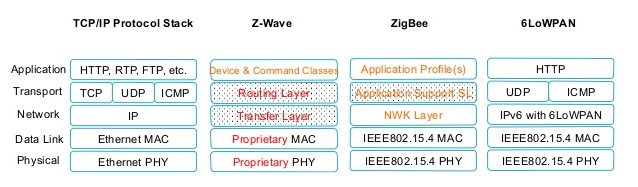
\includegraphics[width=15cm]{\rpDossier/images/comparison.jpg}
\caption{Comparaison de différents protocoles IoT}
\label{comparison}
\end{figure}

-------Mettre des observations pour zigbee et z-wave ?-------

En réalité IPv6 est plus une couche 2.5 que 3, en effet la couche 3 est IPv6. En fait, dans le cas de 6LowPAN la stack réseau ressemble plus à cela :

\begin{figure}[H]
\centering
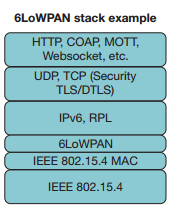
\includegraphics[width=5cm]{\rpDossier/images/stack6lowpan.PNG}
\caption{Stack 6LoWPAN}
\label{stack6lowpan}
\end{figure}

Comme nous pouvons voir, 6LoWPAN fait la liaison entre 802.15.4 et IPv6. Au niveau transport, 6LoWPAN supporte UDP et TCP mais ce dernier n'est pas beaucoup utiliser. En effet, TCP étant un protocole connecté les en-tête sont très grandes (à cause de l'ajout de numéro de séquence par exemple) et donc pas vraiment pratiques pour les appareils basse consommation. Le trafic supplémentaire, avec les ACK, rend son utilisation délicate. On privilégiera plutôt UDP et sa propre version de TLS, DTLS. 

Au niveau applicatif, il est bon de noter que 6LoWPAN supporte HTTP, mais ne l'utilise que très peux a cause de la verbosité du langage. L'industrie a développé un protocole de messagerie plus adapté au nom de \textbf{COAP} (\textit{COnstrained Application Protocol}) qui est beaucoup plus adapté aux appareils basse consommation.

% Compression des en-tête %

% Routage %

% Autoconfiguration %

L'un des avantages d'IPv6 est l'auto-gestion des adresses, un appareil peut générer automatiquement son adresse sans avoir recours à un DHCP. Le protocole \textbf{NDP} (\textit{Neighbor Discovery Protocol}) permet d'obtenir cette adresse unique dans le réseau, ce qui évitera les conflits.

% Securité %

La sécurité dans l'IoT est un véritable challenge, en effet, à cause du nombre de nœuds avec des performances assez faible, il y beaucoup de point d'entré pour les attaques de l'extérieur. Aussi l'un des points critiques dans l'IoT est la nature des données, qui dans certains cas peuvent être cruciale sur elles servent à commander des alarmes ou des portes d'accès.

Du coup, 6LoWPAN tire partie de l'\textbf{AES-128} qui est définie dans 802.15.4. Avec l'utilisation de TLS ou de DTLS on peut aussi sécuriser les échanges au niveau de la couche transport. Mais cela implique d'avoir des équipements avec une certaine puissance. Les cartes TI fournis par notre tuteur ont été développé spécialement dans cette optique de sécurité (\textbf{cc2538}).